\documentclass{beamer}
\usepackage{hyperref}
\usepackage{parskip}
\usepackage{verbatim}
\usepackage{tabularx}
% \usetheme{Madrid}
\usetheme{Boadilla}
% \usetheme{Montpellier}
\usepackage{Sweave}
\begin{document}
\Sconcordance{concordance:Lecture_1.1.tex:Lecture_1.1.Rnw:%
1 8 1 1 0 1774 1}


\title{Intro to R BootCamp Day 1 }
\author{Steve Pittard wsp@emory.edu}
\subtitle{Lecture 1}
\date{\today}

\maketitle

% Section Intro

\section{Intro}

\begin{frame}[fragile]
\frametitle{Why R ? }
\begin{block}{Occupational Outlook Handbook 2014}
Employment of computer and information research scientists is projected to grow 18 percent from 2012 to 2022, faster than the average for all occupations. Employment of statisticians is projected to grow 27 percent from 2012 to 2022, much faster than the average for all occupations. 
\newline
\\
Rapid growth in data collection by businesses may lead to an increased need for data mining services
Information research scientists are likely to enjoy excellent job prospects. 
\newline
\\
Graduates with a master's degree in statistics and a strong background in a related discipline, such as finance, biology, engineering, or computer science, are projected have the best prospects of finding jobs in their field of study.
\end{block}
\end{frame}

% Occupational Outlook 

\begin{frame}[fragile]
\frametitle{Why R ? }
\begin{center}
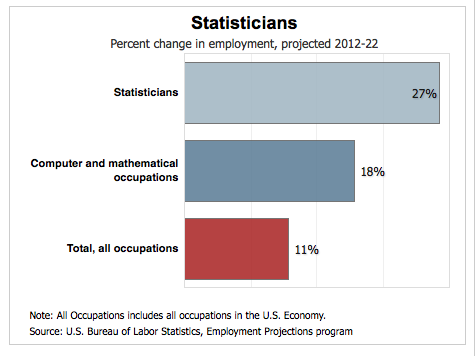
\includegraphics{../IMG/statmath.png}
\end{center}
\end{frame}

% New York Times splash

\begin{frame}[fragile]
\frametitle{New York Times}
\begin{center}
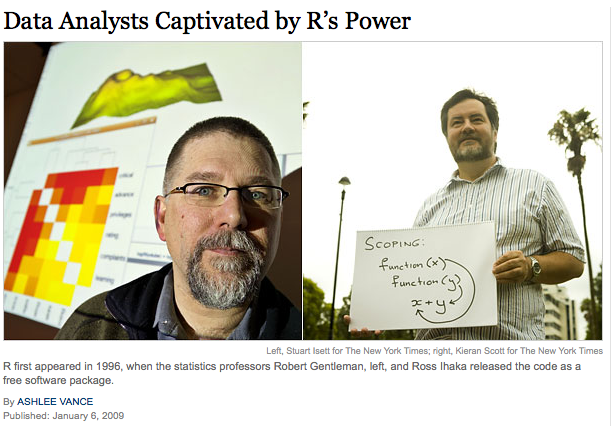
\includegraphics{../IMG/nytimes.png}
\scriptsize
\end{center}
\url{http://tinyurl.com/cxa774n}
\end{frame}

% Companies that use R

\begin{frame}[fragile]
\frametitle{Who Uses R ? }
\small
\begin{center}
\begin{tabular}{| l | l |}
  \hline         
  \textbf{Company} & \textbf{How R is Used} \\ \hline
  Bank of America & Modeling and visualization \\ \hline
  Facebook & User analysis and interaction  \\ \hline
  FDA & Used in parallel with SAS \\ \hline
  Ford Motor Company & Decision support \\ \hline
  Google & Calculate ROI on advertising \\ \hline
  John Deere & Time series modeling and geospatial analysis \\ \hline
  National Weather Service & Visualization for flood forecasting \\ \hline
  New York Times Newspaper & Data visualization \\ \hline
  Nordstrom & Recommendation systems \\ \hline
  Orbitz Travel & Search result optimization \\ \hline
  Twitter & User experience analysis \\ \hline
  Trulia Real Estate & Housing cost predictions \\ \hline
  OK Cupid Online Dating & Trend analysis \\ \hline
  Lloyd's of London Insurance & Investment recommendation \\ \hline
  \hline  
\end{tabular}
\end{center}
\footnotesize
\url{http://www.revolutionanalytics.com/companies-using-r}
\end{frame}

% R compared to other languages

\begin{frame}[fragile]
\frametitle{Why R ? }
\small
\begin{itemize}
\item R is an interactive framework for data and statistical analysis that also happens to have a builtin programming language. 
\item Compare this to languages such as Python, Perl, and Java that have data analysis addons
\item Which language to use ? Use them all if necessary but if data analysis is a large part of the work then R is the ``go to'' language
\item R can reference or call code written in C, C++, Perl, Python, Java, and FORTRAN.
\item Most of the effort in using R relates to shaping data for analysis and understanding the available functions and packages. 
\item To be a good \emph{programmer} in R one must first be a knowledgeable \emph{user} of R. 
\end{itemize}
\end{frame}

% R compared to other languages

\begin{frame}[fragile]
\frametitle{Why R ? }
\small
\begin{block}{Differences between R and other statistical packages}

``When talking about user friendliness of computer software I like to the analogy of cars vs. busses. Using this analogy programs like SPSS are busses, easy to use for the standard things, but very frustrating if you want to do something that is not already preprogrammed.''
\newline
\\
``R is a 4-wheel drive SUV with a bike on the back, a kayak on the top, good walking and running shoes in the passenger seat, and a mountain climbing and spelunking gear in the back.''
\newline
\\
``R can take you anywhere you want to go if you take the time to learn how to use the equipment, but that is going to take longer than learning where the bus stops are in SPSS.''
\newline
\\
Greg Snow, R-help (May 2006)
\end{block}
\end{frame}

% R compared to other languages

\begin{frame}[fragile]
\frametitle{Why R ? }
\small
\begin{block}{Cool things about R}
\begin{itemize}
\item Vast capabilities with a wide range of statistical and graphics techniques
\item Written primarily by statisticians 
\item Free of cost 
\item Collaborative development with over 6,092 user contributed packages
\item Excellent community support with mailing lists, blogs, and tutorials
\item Excellent ``google'' support
\item Wildly popular in Academia and increasingly so in the business world
\end{itemize}
\end{block}
\begin{center}
\url{www.slideshare.net/izahn/rintro}
\end{center}
\end{frame}

% R vs. SAS

\begin{frame}[fragile]
\frametitle{R vs Other Languages - kdnuggets.com}
\begin{center}
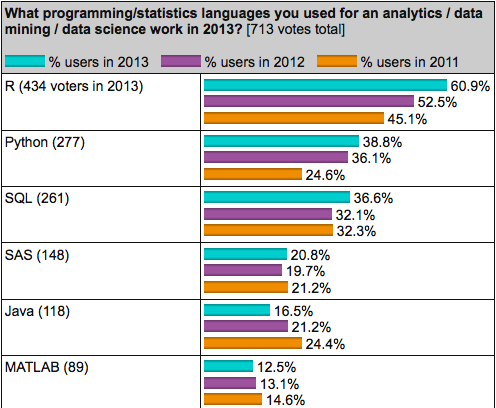
\includegraphics{../IMG/rvsothers.png}
\end{center}
\end{frame}

% Obtaining R

\begin{frame}[fragile]
\frametitle{Obtaining R}
\small
\begin{itemize}
\item Go to \url{http://cran.revolutionanalytics.com/}
\item Click on your platform which will be either Windows or Apple OSX
\item You will be redirected to another page which has a download link near the top
\item Click it to download and begin installation. Wait till it is finished
\item Go to \url{http://www.rstudio.com/products/rstudio/download/} to download the RStudio GUI
\item Double click the installer to initiate the installation of RStudio
\item Once finished start up Rstudio
\end{itemize}
\end{frame}


\section{Packages}

% Base Packages

\begin{frame}[fragile]
\frametitle{Base Packages}
It is important to note that R comes with a base set of packages as part of every installation. 
\newline
\\
\scriptsize
\begin{verbatim}
> getOption("defaultPackages")
[1] "datasets"  "utils"     "grDevices" "graphics"  "stats"     "methods"  

> search()
[1] ".GlobalEnv"        "package:stats"     "package:graphics"  "package:grDevices" 
[5] "package:utils"     "package:datasets"   "package:methods"   "Autoloads"         
[9] "package:base"     

> library(help="stats")
\end{verbatim}
\end{frame}


% Base Packages

\begin{frame}[fragile]
\frametitle{Base Packages}
\scriptsize
\begin{verbatim}
> library(help="stats")
Description:

Package:       stats
Version:       3.1.2
Priority:      base
Title:         The R Stats Package
Author:        R Core Team and contributors worldwide
Maintainer:    R Core Team <R-core@r-project.org>
Description:   R statistical functions
License:       Part of R 3.1.2
Built:         R 3.1.2; x86_64-apple-darwin13.4.0; 2014-10-31 20:19:14 UTC; unix

Index:

.checkMFClasses         Functions to Check the Type of Variables passed
                        to Model Frames
AIC                     Akaike's An Information Criterion
ARMAacf                 Compute Theoretical ACF for an ARMA Process
ARMAtoMA                Convert ARMA Process to Infinite MA Process
Beta                    The Beta Distribution
Binomial                The Binomial Distribution
Box.test                Box-Pierce and Ljung-Box Tests
C                       Sets Contrasts for a Factor
\end{verbatim}
\end{frame}


% Base Packages

\begin{frame}[fragile]
\frametitle{Base Packages}
Many packages come with example data that is helpful when attempting to understand how various functions work. To see what data sets are available in a given package, do something like:
\scriptsize
\begin{verbatim}
> search()
[1] ".GlobalEnv" "package:lattice" "package:stats" "package:graphics" 
[5] "package:grDevices" "package:utils" "package:datasets" "package:methods" 
[9] "Autoloads" "package:base"

> data(package="stats")  # Find data included in package "stats"

Data sets in package "datasets":
AirPassengers           Monthly Airline Passenger Numbers 1949-1960
BJsales                 Sales Data with Leading Indicator
BJsales.lead (BJsales)  Sales Data with Leading Indicator
BOD                     Biochemical Oxygen Demand
CO2                     Carbon Dioxide Uptake in Grass Plants
DNase                   Elisa assay of DNase
EuStockMarkets          Daily Closing Prices of Major European
..
\end{verbatim}
\end{frame}


% Base Packages

\begin{frame}[fragile]
\frametitle{CRAN Packages}
One of the most powerful aspects of R is the ability to install user-contributed addon packages available in CRAN, (Comprehensive R Archive Network). As of December 2014 there are over 6,000 packages available. 
\newline
\\
To obtain information on the wide variety of packages then vist the following URL to see some of the areas covered. \url{cran.cnr.berkeley.edu} Also go to the ``Task Views' You can also see packages grouped by domain at \url{http://cran.r-project.org/web/views/}

\end{frame}

% Addon Packages

\begin{frame}[fragile]
\frametitle{CRAN Packages}
Here are some of the areas covered. There are many more of course
\newline
\\
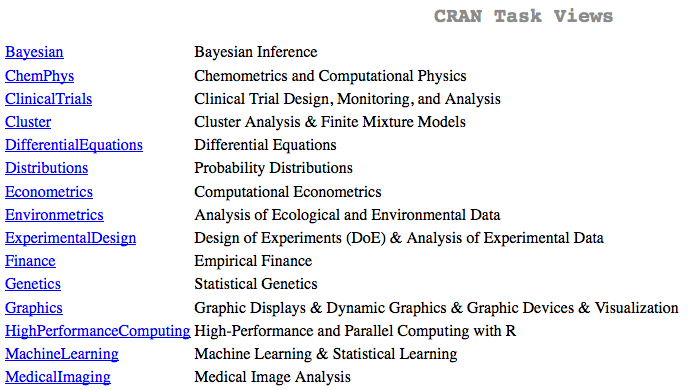
\includegraphics{../IMG/taskviews.png}
\end{frame}

% Addon Packages

\begin{frame}[fragile]
\frametitle{CRAN Packages}
If you are using RStudio there are menu items that can simplify the process of identifying and installing packages. However, you can  also do this from the command prompt. Let's say you want to install the ``actuar'' package from CRAN.
\newline
\\
\footnotesize
\begin{verbatim}
> install.packages("actuar",dependencies=TRUE)

trying URL 'http://mirrors.nics.utk.edu/cran/bin/macosx/contrib/2.15/
actuar_1.1-5.tgz'
Content type 'application/x-gzip' length 1837121 bytes (1.8 Mb)
opened URL
==================================================

downloaded 1.8 Mb
> library(actuar) # Brings the package into the workspace
\end{verbatim}
\end{frame}

% Addon Packages

\begin{frame}[fragile]
\frametitle{CRAN Packages}
When we use the \textbf{library} command to load the contents of the \textbf{actuar} package it will show up when we execute the \textbf{search()} function. Check it out.
\\
\footnotesize
\begin{verbatim}
> library(actuar) # Brings the package into the workspace

> search()

[1] ".GlobalEnv" "package:actuar" "package:lattice" "package:stats" 
[5] "package:graphics" "package:grDevices" "package:utils" 
[8] "package:datasets" "package:methods" "Autoloads" "package:base"
\end{verbatim}
\end{frame}

% omegahat

\begin{frame}[fragile]
\frametitle{CRAN Packages}
On occasion you will need to install a package from a specific repository such as \url{omegahat.org} or R-forge. RStudio has menu items that can help with this but you can also do it from the command line. 
\newline
\\
\footnotesize
\begin{verbatim}
> install.packages("GeoIP", repos = "http://www.omegahat.org/R")
\end{verbatim}
\normalsize
Sometimes you download packages written by colleagues and you have to install them from your local hard drive. Again, RStudio can help but you could also do something like:
\newline
\begin{verbatim}
$ R CMD INSTALL GeoIP.tar.gz
\end{verbatim}
\end{frame}


% CRAN Packages

\begin{frame}[fragile]
\frametitle{CRAN Packages}
There are lots of free books and tutorials on the web.
\newline
\\
\footnotesize
\begin{verbatim}
> install.packages("GeoIP", repos = "http://www.omegahat.org/R")
\end{verbatim}
\normalsize
Sometimes you download packages written by colleagues and you have to install them from your local hard drive. Again, RStudio can help but you could also do something like:
\newline
\begin{verbatim}
$ R CMD INSTALL GeoIP.tar.gz
\end{verbatim}
\end{frame}


\section{Documentation}
% Finding documentation

\begin{frame}[fragile]
\frametitle{Finding Documentation}
There are lots of free books on the web
\newline
\scriptsize

\begin{tabular}{| l | l |}
  \hline         
  \textbf{Resource} & \textbf{URL} \\ \hline
  The R Inferno & \url{http://www.burns-stat.com/documents/books/the-r-inferno/} \\ \hline
  R Programming Wiki & \url{http://en.wikibooks.org/wiki/R_Programming}  \\ \hline
  Intro to Stats Using R & \url{http://ipsur.org} \\ \hline
  Stats with R & \url{http://zoonek2.free.fr/UNIX/48_R/all.html} \\ \hline
  Lattice Graphics & \url{http://lmdvr.r-forge.r-project.org} \\ \hline
  Contributed R Info & \url{http://cran.r-project.org/other-docs.html} \\ \hline
  simpleR Intro Stats & \url{http://cran.r-project.org/doc/contrib/Verzani-SimpleR.pdf} \\ \hline
  DIY Intro to R & \url{http://www.unt.edu/rss/class/Jon/R_SC/} \\ \hline
  R Bloggers & \url{http://www.r-bloggers.com/} \\ \hline
  R Journal & \url{http://journal.r-project.org/} \\ \hline
  R Tutorial & \url{http://www.r-tutor.com/r-introduction} \\ \hline
  Google Style Guide & \url{https://github.com/hadley/devtools/wiki/Style} \\ \hline
  Applied Epi Using R & \url{http://www.medepi.net/docs/EpidemiologyUsingR.pdf} \\ \hline
  \hline  
\end{tabular}
\end{frame}


% Finding documentation

\begin{frame}[fragile]
\frametitle{Finding Documentation}
There are some good books you can buy although for this class they aren't required.
\newline
\footnotesize

\begin{tabular}{| l | l |}
  \hline         
  \textbf{Book} & \textbf{Author} \\ \hline
  R Cookbook & Paul Teetor \\ \hline
  R in a Nutshell & Joseph Adler \\ \hline
  The Art of Programming & Norman Matloff \\ \hline
  Data Manipulation with R & Phil Spector \\ \hline
  ggplot2: Elegant Graphics for Data Analyses & Hadley Wickham \\ \hline
  Intro to Scientific Programming and Simulation Using R & Jones, Maillardet, Robinson \\ \hline
  Introductory Statistics with R & Peter Dalgaard \\ \hline
  The R Book & Michael J. Crawley \\ \hline
  Discovering Statistics Using R & Andy Field \\ \hline
  \hline  
\end{tabular}

\end{frame}

% Mailing Lists

\begin{frame}[fragile]
\frametitle{Mailing Lists}
\begin{itemize}
\item Here are some mailing lists that accept questions relative to R and BioConductor. 
\item Moderators and participants in these lists take questions seriously, sometimes too seriously, \item Please don't ask a question without first searching through the archives to see if your question has already been answered. Chances are it has.
\end{itemize}
\small

\begin{center}
\begin{tabular}{| l | l |}
  \hline         
  \textbf{Mailing Lists} & \textbf{URL} \\ \hline
  R-Help & \url{http://stat.ethz.ch/mailman/listinfo/r-help} \\ \hline
  Cross Validated & \url{http://stats.stackexchange.com} \\ \hline
  Stack Overflow & \url{http://stackoverflow.com/questions/tagged} \\ \hline
  \hline  
\end{tabular}
\end{center}
\end{frame}


% Getting Help

\begin{frame}[fragile]
\frametitle{Getting Help}
R has a number of ways to get help. Rstudio has a Help menu item. Other ways include the following:
\footnotesize
\begin{verbatim}
> help.start()         # Launches a web browser with search capability

> help(function_name)  # Get help on "function_name"

>?function_name        # Equivalent to the above

> args(function_name)    # See what arguments the function accepts

> example(function_name) # See an example of the function

> example(mean)

mean> x <- c(0:10, 50)
mean> xm <- mean(x)
mean> c(xm, mean(x, trim = 0.10))
[1] 8.75 5.50
\end{verbatim}
\end{frame}


% Getting Help

\begin{frame}[fragile]
\frametitle{Getting Help}
R has a number of ways to get help. Rstudio has a Help menu item. Other ways include the following:
\scriptsize
\begin{verbatim}
# Find all functions and data having to do with time series

> help.search("time series") 

>??"time series"    # Equivalent to the above

Help files with alias or concept or title matching "time series" 
using fuzzy matching:

boot::tsboot          Bootstrapping of Time Series
datasets::austres     Quarterly Time Series of the Number of Australian Residents
datasets::beavers     Body Temperature Series of Two Beavers
ggplot2::economics    US economic time series.
lattice::xyplot.ts    Time series plotting methods
MASS::beav1           Body Temperature Series of Beaver 1
MASS::beav2           Body Temperature Series of Beaver 2
stats::StructTS       Fit Structural Time Series
stats::ar             Fit Autoregressive Models to Time Series
stats::ar.ols         Fit Autoregressive Models to Time Series by OLS
..
\end{verbatim}
\end{frame}


% Getting Help

\begin{frame}[fragile]
\frametitle{Things to Know !}
\begin{itemize}
\item Everything in R is an object
\item The great thing about R is that there are many different ways to do something
\item The bad thing about R is that there are many different ways to do something
\item Everything that happens in R is a function call
\item Supports procedural programming with functions and object oriented programming 
\item R is based on a ``read-eval-print'' loop
\item Interpreted langauge
\end{itemize}

\end{frame}

\section{Basic Example Walkthrough}
% Walkthrough

\begin{frame}[fragile]
\frametitle{Walkthrough}
\scriptsize
\begin{verbatim}
url <- "http://steviep42.bitbucket.org/YOUTUBE.DIR/table_7_3.csv"

engine <- read.table(url, sep = ",", header=TRUE)
engine <- engine[,-1]

head(engine) # 3 engine pollutants

    hc co nox
1 0.50 5.01 1.28
2 0.65 14.67 0.72
3 0.46 8.60 1.17
4 0.41 4.42 1.31
5 0.41 4.95 1.16

summary(engine)
     en hc co nox
Min.   : 1.00   Min.   :0.3400   Min.   : 1.850  Min.   :0.490
1st Qu.:12.75   1st Qu.:0.4375   1st Qu.: 4.388  1st Qu.:1.110
Median :24.50   Median :0.5100   Median : 5.905  Median :1.315
Mean   :24.00   Mean   :0.5502   Mean   : 7.879  Mean   :1.340
3rd Qu.:35.25   3rd Qu.:0.6025   3rd Qu.:10.015  3rd Qu.:1.495
Max.   :46.00   Max.   :1.1000   Max.   :23.530  Max.   :2.940
\end{verbatim}
\scriptsize
\url{http://www.cyclismo.org/tutorial/R/hwI.html}

\end{frame}


% Walkthrough

\begin{frame}[fragile]
\frametitle{Walkthrough}

\footnotesize
\begin{verbatim}
boxplot(engine,col="red",main="Engine Pollutants")

\end{verbatim}
\begin{center}
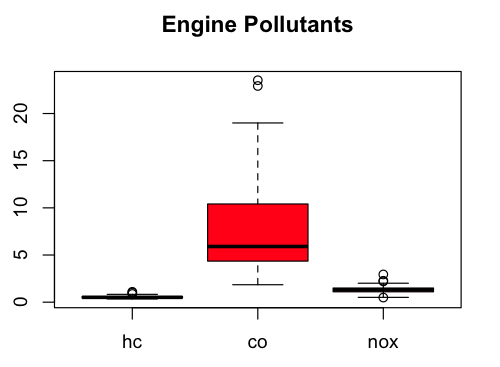
\includegraphics[height=7cm]{../IMG/pollute.png}
\end{center}
\end{frame}

% Walkthrough

\begin{frame}[fragile]
\frametitle{Walkthrough}

\small
\begin{verbatim}
par(mfrow=c(1,3))

boxplot(engine$co,main="Carbon Monoxide")

hist(engine$co)

qqnorm(engine$co,main="Carbon Monoxide")

qqline(engine$co)

\end{verbatim}
\begin{center}
\end{center}
\end{frame}

% Walkthrough

\begin{frame}[fragile]
\frametitle{Walkthrough}

\begin{center}
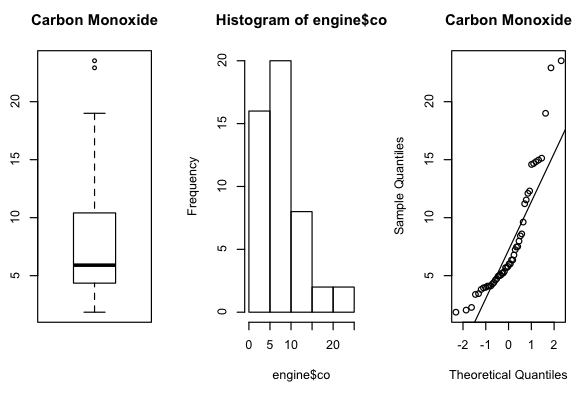
\includegraphics[width=12cm,height=7cm]{../IMG/3plot.png}
\end{center}
\end{frame}

% Walkthrough

\begin{frame}[fragile]
\frametitle{Walkthrough}
\footnotesize
\begin{verbatim}
# The null hypothesis is that the data is normal

shapiro.test(engine$co)

   Shapiro-Wilk normality test

data: engine$co
W = 0.8357, p-value = 9.289e-06

# Take the log of the CO

log.engine <- log(engine$co)

shapiro.test(log.engine)

  Shapiro-Wilk normality test
  
data: log.engine
W = 0.9693, p-value = 0.2379
\end{verbatim}
\end{frame}

% Walkthrough

\begin{frame}[fragile]
\frametitle{Walkthrough}
\small
\begin{verbatim}
par(mfrow=c(2,2))

log.engine <- log(engine$co)

boxplot(log.engine,main="Carbon Monoxide")

hist(log.engine,main="Carbon Monoxide")

qqnorm(log.engine,main="QQ Plot for the Log of the 
                        Carbon Monoxide")

qqline(log.engine)
\end{verbatim}
\end{frame}

% Walkthrough

\begin{frame}[fragile]
\frametitle{Walkthrough}
\begin{center}
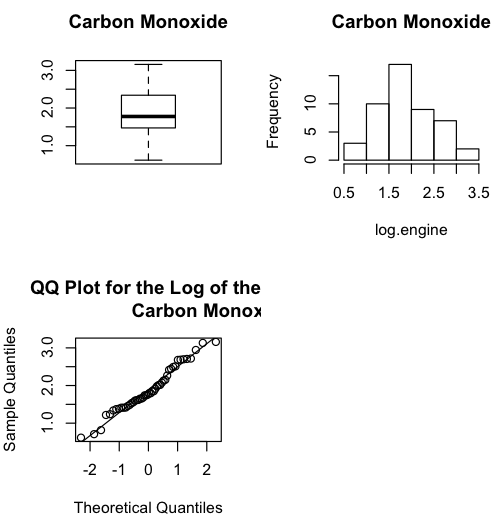
\includegraphics[height=8cm]{../IMG/walk2.png}
\end{center}
\end{frame}



% Walkthrough

\begin{frame}[fragile]
\frametitle{Walkthrough}
\footnotesize
\begin{verbatim}
# Let's build a confidence interval

my.mean <- mean(log.engine)
my.sd < sd(log.engine)
n <- length(log.engine)

# Get standard error
se <- my.sd/sqrt(n)

error <- se*qt(0.975,df=n-1)

left <- my.mean - error

right <- my.mean + error

c(left,right)
[1] 1.709925 2.057431

c(exp(left),exp(right))
[1] 5.528548 7.825840
\end{verbatim}
\end{frame}

% Walkthrough

\begin{frame}[fragile]
\frametitle{Walkthrough}
\footnotesize
\begin{verbatim}
# Test H0: mu = 5.4
# HA:mu != 5.4

lNull <- log(5.4) - error

rNull <- log(5.4) + error

c(lNull,rNull)
[1] 1.512646 1.860152

my.mean
[1] 1.883678
\end{verbatim}
\small
So the mean is outside the range thus we reject the null. There is a low probability that we would have obtained our sample mean if the true mean really was 5.4
\end{frame}

% Walkthrough

\begin{frame}[fragile]
\frametitle{Walkthrough}
\small
We could have calculated a p-value by hand
\begin{verbatim}
p.val <- 2*(1-pt((my.mean-log(5.4))/se,df=n-1))

p.val
[1] 0.02692539

# But its easier to call a procedure to do it all !!!!

t.test(log.engine,mu = log(5.4),alternative = "two.sided")
   One Sample t-test
data: log.engine
t = 2.2841, df = 47, p-value = 0.02693
alternative hypothesis: true mean is not equal to 1.686399
95 percent confidence interval:
  1.709925 2.057431
sample estimates:
mean of x
1.883678
\end{verbatim}
\end{frame}

\section{First Session}

% First R session

\begin{frame}[fragile]
\frametitle{First R Session}
\footnotesize
\begin{verbatim}
?mean             # Get help on the mean function

example(kmeans)   # Run an example of kmeans (if it exists)

pi                # Some popular quantities are built-?‐in to R
[1] 3.141593

sqrt(2) # Basic arithmetic
[1] 1.414214

print(pi) # Print the comments of the pi variable
[1] 3.141593

X <- 3; Y <- 4 # Semicolon lets you enter 2 commands on the same line

Z <- sqrt(X^2 + Y^2) # Variables contain information

# List all variables in the "environment"

ls()
[1] "X" "Y" "Z"
\end{verbatim}
\end{frame}

% First R session

% Finding documentation
\begin{frame}[fragile]
\footnotesize
\begin{verbatim}
log(10)             ceiling(6.8)             2+3
[1] 2.302585        [1] 7                    [1] 5

log10(100)          round(6.889,2)           3/2
[1] 2               [1] 6.89                 [1] 1.5

sin(pi/2)           3/0                      2^3 
[1] 1               [1] Inf                  [1] 8
 
cos(pi/2)           0/0                      (56-14)/6 - 4*7*10/(5^2-5)
[1] 6.123234e-17    [1] NaN                  [1] -7

1.3e6               is.finite(3)             abs(2-4)
[1] 1300000         [1] TRUE                 [1] 2

9 %% 2              x <- c(1:8,NA)           
[1] 1               [1] 1 2 3 4 5 6 7 8 NA

floor(5.7)          mean(x)
[1] 5               NA
\end{verbatim}
\end{frame}

% Common logical operators

\begin{frame}[fragile]
\frametitle{Common Operators}
\scriptsize
\begin{verbatim}
# RELATIONAL OPERATORS

Equal to               ==           if (myvar == "test") {print("EQ")} 
                       ==           if (mnynum == 3)     {print("EQ")} 
Not equal to           !=           if (myvar != "test") {print("NE")} 
Less than or equal to  <=           if (number <= 5)     {print("LTE")}
Less than              <            if (number < 10)     {print("LT")}
Greater than or equal to  >=        if (number >= 10)    {print("GTE")}
Greater than              >         if (number > 12)     {print("GT")}

# BOOLEAN OPERATORS 

And                    &      if ((myvar == "test") & (num <= 10) ) { 
                                     print("Equal and less than")
                              }
                                     
Not                    !      if (!complete.cases(myvec)) {
                                     print("Non complete cases")
                              } 

Or                     |      if ((num > 3) | (num < -3)) {
                                     print("Only one of these has to be true")
                              }
\end{verbatim}
\end{frame}


% Common logical operators

\begin{frame}[fragile]
\frametitle{More Examples}
Here are some popular math formulas rewritten in R. Note that the variables must first exist in order for the formula to do an actual computation.
\scriptsize

\begin{verbatim}
# a^2 + b^2 = c^2                 # Pythagorean Theorem

a <- 2; b <- 4

c <- sqrt(a^2 + b^2)              # To solve the PT for c

a <- 2; b <- 4; c <- 1

(-b + sqrt(b^2-4*a*c)) / (2*a)    # First case quadratic formula solution

(-b - sqrt(b^2 - 4*a*c)) / (2*a)  # Second case quadratic formula solution
r <- 4; h <- 6; b <- 3

circumference <- 2*pi*r             # circumference of a circle

area <- (b*h)/2 # Area of a triangle  
\end{verbatim}
\end{frame}

\section{Functions}

\begin{frame}[fragile]
\frametitle{Expressions}
We can create functions that contain resuable code for later use 
\small

\begin{verbatim}
my.quad <- function(a,b,c) {
  r1 <- (-b + sqrt(b^2 - 4*a*c)) / (2*a)
  r2 <- (-b - sqrt(b^2 - 4*a*c)) / (2*a)
  my.roots = c(r1,r2)
  return(my.roots)
}

# Solve for ax^2 + bx + c where a = 1, b=6, and c=8

my.quad(1,6,8)

\end{verbatim}
\end{frame}

% Workspace

\section{Workspace and Environment}

\begin{frame}[fragile]
\frametitle{Startup}
\begin{itemize}

\item You can use the Preferences menu item in RStudio to specify your default home directory

\item When R starts it looks for a file called .Rprofile within your home directory

\item You can influence the R environment by setting a number of ``startup'' variables therein

\item Use your favorite editor to create/edit this file in your default folder

\item You can change many of these variables or options during an R session but if you want them to 
be permanent then you will need to edit the .Rpfofile file

\end{itemize}

\end{frame}


% Workspace

\begin{frame}[fragile]
\frametitle{Startup .Rprofile}
\scriptsize
\begin{verbatim}
# Things you might want to change

options(editor="notepad")
cd = setwd
pwd = getwd
lss = dir

# R interactive prompt
setwd("/Users/fender/steve.test") # Set's my default directory for me.
options(prompt="> ")
options(continue="+ ")

# General options
options(digits=3)
options(width = 130)
options(graphics.record=TRUE)
.First <- function(){             # You can load functions
library(Hmisc)
cat("\nWelcome at", date(), "\n")
}
.Last <- function(){
cat("\nGoodbye at ", date(), "\n")
}
\end{verbatim}
\end{frame}


\begin{frame}[fragile]
\frametitle{Workspace - Being Organized}
Being organized helps ! Knowing how to find stuff quickly is essential. Create a master folder that will contain your work in this class. 
\newline
\\
You can create subfolders according to your projects. Note that some people do this on a DropBox folder to insure that all work is backed up.  
\\
\footnotesize
\begin{verbatim}
$ ls RProjects
RProjects
    Data_Files
    Genomes
            1000_Genomes
            Centenarians
    HIV
            Replicates
    Hepatitis
            Hep_A
            Hep_B
\end{verbatim}
\end{frame}
% Workspace - Navigating Directories

\begin{frame}[fragile]
\frametitle{Workspace - Navigating Directories}
There are a number of functions that allow you to ``move'' around in your folder structure. These are important to know because sometimes you will need to write code that needs to refer to specific folders and files during execution.
\scriptsize
\begin{verbatim}
getwd()
[1] "/Users/fender/TEST.DIR"

setwd("/Users/fender")
getwd()
[1] "/Users/fender"

setwd("/Users/fender/TEST.DIR")
getwd()
[1] "/Users/fender/TEST.DIR"

dir()
[1] "coolpkg" "coolpkg_1.0.tar.gz" "coolpkg.pdf" "coolpkg.Rcheck"
"g.Rd" "stuff.R"
\end{verbatim}
\end{frame}


% Workspace - Navigating Directories

\begin{frame}[fragile]
\frametitle{Workspace - Listing Files}
R also has some functions that list files in a folder. You can do this visually within R Studio although sometimes you will need to use these commands to open and read in files as part of a program.
\footnotesize
\begin{verbatim}
myfiles <- list.files()

str(myfiles)
 chr [1:29] "001.csv" "002.csv" "003.csv" "004.csv" "005.csv" "006.csv" ... 

myfiles[1:5]
[1] "001.csv" "002.csv" "003.csv" "004.csv" "005.csv"
 
# You could write a for-loop to process each and every file

for (ii in 1:length(myfiles)) {
    file <- myfiles[ii]
    # Do something 
} 
\end{verbatim}
\end{frame}

% Workspace - Saving Workspace

\begin{frame}[fragile]
\frametitle{Workspace - ls()}
R creates an environment for each session you initiate. This is very useful because it accumulates all your variables and objects while you experiment with data. 
\newline
\\
Over time your environment will accumulate lots of variables. In general this is good because you don't lose anything. The \textbf{ls()} function can show you what objects you currently have in your environment.
\scriptsize
\begin{verbatim}
ls()
 [1] "access_log"                       "cntr"                            
 [3] "ii"                               "init"                            
 [5] "mpg"                              "mtcars"                          
 [7] "mymean"                           "myrle"                           
 [9] "mystr"                            "nhanes1"                         
[11] "retvec"                           "retvectr"                        
[13] "SacramentocrimeJanuary2006"       "Sacramentorealestatetransactions"
[15] "SalesJan2009"                    
\end{verbatim}
\end{frame}

\begin{frame}[fragile]
\frametitle{Workspace - rm()}
You can remove one or more objects using the \textbf{rm()} function
\footnotesize
\begin{verbatim}
ls()
 [1] "access_log"                       "cntr"                            
 [3] "ii"                               "init"                            
 [5] "mpg"                              "mtcars"                          
 [7] "mymean"                           "myrle"                           
 [9] "mystr"                            "nhanes1"                         
[11] "retvec"                           "retvectr"                        
[13] "SacramentocrimeJanuary2006"       "Sacramentorealestatetransactions"
[15] "SalesJan2009"                    

rm(access_log)    # Removes the object named "access_log"

access_log        # Now R can't find it
Error: object 'access_log' not found

rm(mystr,retvec,init)     # Remove more than one object at once
\end{verbatim}
\end{frame}

% Workspace - Saving Workspace

\begin{frame}[fragile]
\frametitle{Workspace - .Rdata}
When you quit R you will be asked if you wish to save your current environment to disk. If you type ``y'' then all objects, (and their values), will be written to a file called \textbf{.Rdata}

This is useful because when you restart R in the same folder it will read \textbf{.Rdata} which contains all previously saved information.
\footnotesize
\begin{verbatim}
> q()
Save workspace image? [y/n/c]: y
Goodbye at Mon Oct 1 14:26:47 2012

fenders-macbook:TEST.DIR fender$ ls .Rdata
.Rdata
\end{verbatim}
\normalsize
The \textbf{.Rdata} file is a ``binary'' file, (its contents are unintelligible to the eye), that contains all the R objects and values in between sessions. This file could be shared with others if you wanted. 
\end{frame}


% Workspace - Saving Workspace

\begin{frame}[fragile]
\frametitle{Workspace - save()}
You can also save one or more objects to a file using the \textbf{save()} function. The inverse of the \textbf{save()} function is the \textbf{load()} function.
\footnotesize
\begin{verbatim}
my.lm <- lm(mpg ~ wt,mtcars)

ls(my.lm)
[1] "assign" "call" "coefficients" "df.residual" "effects" "fitted.values" 
[7] "model"   "qr" "rank" "residuals" "terms" "xlevels"

save(my.lm,file="/Users/myhome/mylmresults")

# You can come back later and load this file

mylmstuff <- load("/Users/myhome/mylmresults")
\end{verbatim}
\end{frame}


% Workspace - Saving Workspace

\section{Variables}

\begin{frame}[fragile]
\frametitle{Variables}
As in most programming languages, it is customary to store or hold the results of an operation
in a variable name. 
\newline
\\
In R such results are assigned with the symbols "\texttt{<-}" or "\textbf{=}". Variable names are case sensitive.
\footnotesize
\begin{verbatim}
A <- 2.5    # The "<-" is the preferred method of assignment

A = 2.5     # This is equivalent to the above although using the "=" is 
            # discouraged except in setting function arguments.

A
[1] 2.5

mynewvar <- X + 3

MYNEWVAR <- X + 3    # Two different variables

\end{verbatim}
\end{frame}


\begin{frame}[fragile]
\frametitle{Variables}
\begin{itemize}
\item R has several one-letter reserved words: c, q, s, t, C, D, F, I, T
\item Variables cannot begin with the period characters ``.''
\item Variable names are case sensitive, so ``myvar'' is different from ``Myvar''
\item Variable names cannot begin with numbers or symbols (\%,\$,\_)
\item Variable names cannot contain spaves in the name ("my var")
\end{itemize}

\end{frame}

% 

\begin{frame}[fragile]
\frametitle{Variables }

\begin{verbatim}
mean.height          .mean.height
smoker               _myvariable
non.smoker           _Mean.height
temp.var             1variable
patient_id           1_variable
Eye.Color            %some.var
State_Population     some.var
disease.state        "some var"
White_Cell_Count     $myvar
jobTitle             
\end{verbatim}

\footnotesize
\end{frame}


\section{Reading and Writing Data}
\begin{frame}[fragile]
\frametitle{Reading and Writing Files }
R has a number of builtin example data frames. One common way to import data is via ``.csv'' files. Before we consider reading a .csv file let's first create one.
\footnotesize
\begin{verbatim}
head(mtcars)
                mpg cyl disp hp drat wt qsec vs am gear carb
Mazda RX4       21.0 6 160 110 3.90 2.620 16.46 0 1 4 4
Mazda RX4 Wag   21.0 6 160 110 3.90 2.875 17.02 0 1 4 4
Datsun 710      22.8 4 108  93 3.85 2.320 18.61 1 1 4 1
Hornet 4 Drive  21.4 6 258 110 3.08 3.215 19.44 1 0 3 1

write.table(mtcars,file="mtcars.csv",
            row.names=TRUE,               # Row names get saved
            col.names=TRUE,               # Header gets saved
            sep=",")                      # Field seperator is ,

$ head mtcars.csv
"mpg","cyl","disp","hp","drat","wt","qsec","vs","am","gear","carb"
"Mazda RX4",21,6,160,110,3.9,2.62,16.46,0,1,4,4
"Mazda RX4 Wag",21,6,160,110,3.9,2.875,17.02,0,1,4,4  
\end{verbatim}

\footnotesize

\end{frame}

%

\begin{frame}[fragile]
\frametitle{Reading and Writing Files }
The first line of mtcars.csv describes the column names. Each subsequent row represents an observation with each field being separated by a ``,''. Let's read it in:
\footnotesize
\begin{verbatim}

mycars <- read.table("mtcars.csv",header=TRUE,sep=",")

head(mycars)
                   mpg cyl disp  hp drat    wt  qsec vs am gear carb
Mazda RX4         21.0   6  160 110 3.90 2.620 16.46  0  1    4    4
Mazda RX4 Wag     21.0   6  160 110 3.90 2.875 17.02  0  1    4    4
Datsun 710        22.8   4  108  93 3.85 2.320 18.61  1  1    4    1
Hornet 4 Drive    21.4   6  258 110 3.08 3.215 19.44  1  0    3    1
Hornet Sportabout 18.7   8  360 175 3.15 3.440 17.02  0  0    3    2
Valiant           18.1   6  225 105 2.76 3.460 20.22  1  0    3    1 
\end{verbatim}
\footnotesize
\end{frame}

\subsection{Reading from the Internet}
%
\begin{frame}[fragile]
\frametitle{Reading Files from an URL}
You can read CSV files from the Internet as long as you know the URL. Here is a simple case
\tiny
\begin{verbatim}
url <- "https://raw.githubusercontent.com/steviep42/bootcamp/master/data/airports.csv"
airports <- read.csv(url)
head(airports)

 faa                           name      lat       lon  alt tz dst
1 04G              Lansdowne Airport 41.13047 -80.61958 1044 -5   A
2 06A  Moton Field Municipal Airport 32.46057 -85.68003  264 -5   A
3 06C            Schaumburg Regional 41.98934 -88.10124  801 -6   A
4 06N                Randall Airport 41.43191 -74.39156  523 -5   A
5 09J          Jekyll Island Airport 31.07447 -81.42778   11 -4   A
6 0A9 Elizabethton Municipal Airport 36.37122 -82.17342 1593 -4   A

\end{verbatim}
\footnotesize
\end{frame}


%
\subsection{Reading in Numbers with Commas}
\begin{frame}[fragile]
\frametitle{Reading Files - Commas}
Sometimes we get numerical data that has delimiters within it. Like with numbers in the thousands.
They can contain commas to offeset every three zeroes. If you make no effort R will think
that they are characters. 
\tiny
\begin{verbatim}
url <- "https://raw.githubusercontent.com/steviep42/bootcamp/master/data/employees.csv"
employees <- read.csv(url,sep="\t")

head(employees)
          name age salary
1  Frank,Smith  34 10,000
2   Jones,Carl  22 12,000
3   Smith,Mary  26 13,000
4 Johnson,Lisa  32 13,500

str(employees)
'data.frame':	4 obs. of  3 variables:
 $ name  : Factor w/ 4 levels "Frank,Smith",..: 1 3 4 2
 $ age   : int  34 22 26 32
 $ salary: Factor w/ 4 levels "10,000","12,000",..: 1 2 3 4
\end{verbatim}
\footnotesize
\end{frame}

%

\begin{frame}[fragile]
\frametitle{Reading Files - Commas}
\begin{itemize}
\item We can use \textbf{coercion} to ``persuade'' a variable that is character to be a numeric variable
\item First we use a function to eliminate the comma since its presence is what makes R think the variable is a character. 
\item Then we use the \textbf{as.numeric()} function to change the variable into a numeric.
\end{itemize}
\tiny
\begin{verbatim}
url <- "https://raw.githubusercontent.com/steviep42/bootcamp/master/data/employees.csv"
employees <- read.csv(url,sep="\t")

employees$salary <- as.numeric(gsub(",","",employees$salary))
 
str(employees)
'data.frame':	4 obs. of  3 variables:
 $ name  : Factor w/ 4 levels "Frank,Smith",..: 1 3 4 2
 $ age   : int  34 22 26 32
 $ salary: num  10000 12000 13000 13500

\end{verbatim}
\footnotesize
\end{frame}

%

%
\subsection{Federal Campaign Contribution Data}
\begin{frame}[fragile]
\frametitle{A Real Example}Check out the Federal Election Commission Website for information on Campaign Contributions by Individuals. There are other types of information also but for now we will look at donations from people.
\newline
\\
\url{http://www.fec.gov/finance/disclosure/ftpdet.shtml}
\newline

\includegraphics{../IMG/election_website.png}
\end{frame}

% 

\begin{frame}[fragile]
\frametitle{A Real Example} If you go to the download link and find the file corresponding to individual contributions you will see that the file has 12,395,164 records. There is also a link to the data dictionary link that you can click.
\newline
\scriptsize
\url{http://www.fec.gov/finance/disclosure/metadata/indiv_header_file.csv}
\normalsize
The size of the file is about 426 Megabytes. We won't work with that. Instead we will work with a prepared file that has information relating only to Georgia. 

\footnotesize
\url{http://www.fec.gov/finance/disclosure/ftpdet.shtml#a2015_2016}
\newline
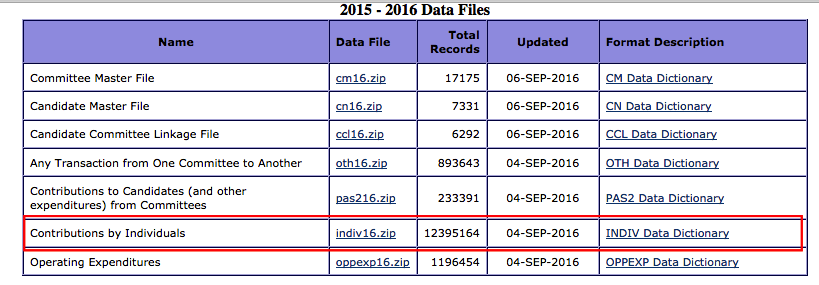
\includegraphics{../IMG/campaign.png}
\end{frame}

% 

\begin{frame}[fragile]
\frametitle{A Real Example}Let's get to work on this file.
\tiny
\begin{verbatim}
url <- "https://raw.githubusercontent.com/steviep42/bootcamp/master/data/georgia_campaign.txt"

# Rather than read it directly from the Internet we'll first download it

download.file(url,"georgia_campaign.txt")

# Let's take a peek at the first three lines

system("head -3 georgia_campaign.txt")

C00076182|N|Q1|P|15951125081|15|IND|JAMES, JIM|HOSCHTON|GA|305481390|MAREL STORK POULTRY PROCESSING|VP OF TECHNICAL SERVICES|03242015|300||A0DAECF187E8D4B41ACF|1002289|||4041320151241796907
C00076182|N|Q1||15951125081|15|IND|JAMES, JIM|HOSCHTON|GA|305481390|MAREL STORK POULTRY PROCESSING|VP OF TECHNICAL SERVICES|03242015|40||A49D962C4ECF047AB97B|1002289|||4041320151241796908
C00186064|N|M4||15970338248|15|IND|NUNNERY, JOHN|COLUMBUS|GA|319062001|PNC BANK NA|SR. VICE PRESIDENT|03312015|100||PR363907910124|1002291||P/R DEDUCTION ($50.00 BI-WEEKLY)|4041320151241796958

# Read it in

gacamp <- read.csv("georgia_campaign.txt",sep="|",header=FALSE, stringsAsFactors=FALSE)

head(gacamp,1)
         V1 V2 V3 V4          V5 V6  V7         V8       V9 V10       V11
1 C00076182  N Q1  P 15951125081 15 IND JAMES, JIM HOSCHTON  GA 305481390

                             V12                      V13     V14 V15 V16
1 MAREL STORK POULTRY PROCESSING VP OF TECHNICAL SERVICES 3242015 300    

1 A0DAECF187E8D4B41ACF 1002289         4.04132e+18
2 A49D962C4ECF047AB97B 1002289         4.04132e+18

\end{verbatim}
\end{frame}

%


\begin{frame}[fragile]
\frametitle{A Real Example}Let's get to work on this file.
\tiny
\begin{verbatim}
url <- "https://raw.githubusercontent.com/steviep42/bootcamp/master/data/indiv_header_file.csv"

# Note the "stringsAsFactors argument

( colnames <- read.csv(url,sep=",",header=F,stringsAsFactors=FALSE) )
       V1        V2     V3              V4        V5             V6        V7
1 CMTE_ID AMNDT_IND RPT_TP TRANSACTION_PGI IMAGE_NUM TRANSACTION_TP ENTITY_TP
    V8   V9   V10      V11      V12        V13            V14             V15
1 NAME CITY STATE ZIP_CODE EMPLOYER OCCUPATION TRANSACTION_DT TRANSACTION_AMT
       V16     V17      V18     V19       V20    V21
1 OTHER_ID TRAN_ID FILE_NUM MEMO_CD MEMO_TEXT SUB_ID

# Let's give each column a more descriptive name

names(gacamp) <- as.vector(colnames[1,])

head(gacamp,1)
    CMTE_ID AMNDT_IND RPT_TP TRANSACTION_PGI   IMAGE_NUM TRANSACTION_TP
1 C00076182         N     Q1               P 15951125081             15
  ENTITY_TP       NAME     CITY STATE  ZIP_CODE                       EMPLOYER
1       IND JAMES, JIM HOSCHTON    GA 305481390 MAREL STORK POULTRY PROCESSING
                OCCUPATION TRANSACTION_DT TRANSACTION_AMT OTHER_ID
1 VP OF TECHNICAL SERVICES        3242015             300         
               TRAN_ID FILE_NUM MEMO_CD MEMO_TEXT      SUB_ID
1 A0DAECF187E8D4B41ACF  1002289                   4.04132e+18

\end{verbatim}
\end{frame}

%

\begin{frame}[fragile]
\frametitle{A Real Example}Let's get to work on this file.
\tiny
\begin{verbatim}
str(gacamp)
'data.frame':	267408 obs. of  21 variables:
 $ CMTE_ID        : chr  "C00076182" "C00076182" "C00186064" "C00508804" ...
 $ AMNDT_IND      : chr  "N" "N" "N" "N" ...
 $ RPT_TP         : chr  "Q1" "Q1" "M4" "Q1" ...
 $ TRANSACTION_PGI: chr  "P" "" "" "P" ...
 $ IMAGE_NUM      : num  1.6e+10 1.6e+10 1.6e+10 1.6e+10 1.6e+10 ...
 $ TRANSACTION_TP : chr  "15" "15" "15" "15E" ...
 $ ENTITY_TP      : chr  "IND" "IND" "IND" "IND" ...
 $ NAME           : chr  "JAMES, JIM" "JAMES, JIM" "NUNNERY, JOHN" "DOWNS, BERTIS" ...
 $ CITY           : chr  "HOSCHTON" "HOSCHTON" "COLUMBUS" "ATHENS" ...
 $ STATE          : chr  "GA" "GA" "GA" "GA" ...
 $ ZIP_CODE       : chr  "305481390" "305481390" "319062001" "30606" ...
 $ EMPLOYER       : chr  "MAREL STORK POULTRY PROCESSING" "MAREL STORK POULTRY PROCESSING" "PNC BANK NA" "N/A" ...
 $ OCCUPATION     : chr  "VP OF TECHNICAL SERVICES" "VP OF TECHNICAL SERVICES" "SR. VICE PRESIDENT" "ATTORNEY" ...
 $ TRANSACTION_DT : int  3242015 3242015 3312015 3302015 2272015 3312015 3032015 3152015 3312015 3272015 ...
 $ TRANSACTION_AMT: int  300 40 100 500 500 2000 1000 2 50 250 ...
 $ OTHER_ID       : chr  "" "" "" "C00401224" ...
 $ TRAN_ID        : chr  "A0DAECF187E8D4B41ACF" "A49D962C4ECF047AB97B" "PR363907910124" "11AI-000046699" ...
 $ FILE_NUM       : int  1002289 1002289 1002291 1003915 1003915 1003922 1003948 1003950 1003950 1002628 ...
 $ MEMO_CD        : chr  "" "" "" "" ...
 $ MEMO_TEXT      : chr  "" "" "P/R DEDUCTION ($50.00 BI-WEEKLY)" "EARMARKED THROUGH ACTBLUE CONDUIT COMMITTEE 03-31-2015  $38,539.37-SEE MEMO ON SCH A FOR LINE 11C" ...
 $ SUB_ID         : num  4.04e+18 4.04e+18 4.04e+18 4.04e+18 4.04e+18 ...
> 


\end{verbatim}
\end{frame}


\subsection{Reading in Tables}
\begin{frame}[fragile]
\frametitle{Reading Tabular Data}
\small
You already know that you can read CSV files directly a URL. But you can also read data directly from a table from a website. Take a look at this example. Let's say we want to get the data from this link on Wikipedia \url{https://en.wikipedia.org/wiki/World_population}. This appears to be the 6th table on the page. 
\begin{center}
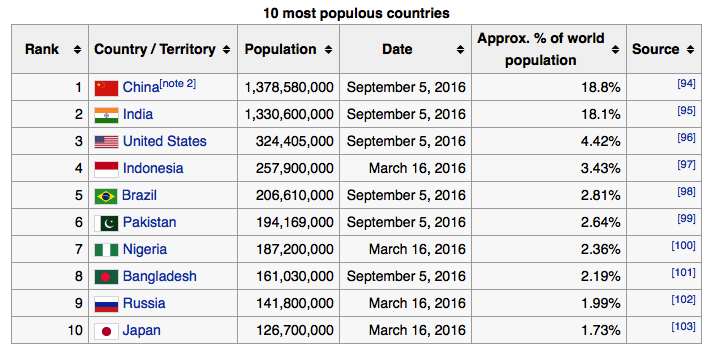
\includegraphics[height=3.5cm,width=6.5cm]{../IMG/world_population_wiki.png}
\end{center}
\end{frame}

%
\begin{frame}[fragile]
\frametitle{Reading Tabular Data}
\footnotesize
\begin{verbatim}
url <- "https://en.wikipedia.org/wiki/World_population"

# The following will "parse" the underlying HTML for the page

my_html <- read_html(url)

# Next we want to get the "nodes" from the parsed HTML that correspond 
# to tables. There are in fact many tables on this page but we are 
# trying to target the one that has the ten most populous countries

my_tables <- html_nodes(my_html,"table")[[6]]

populous_table <- html_table(my_tables)
\end{verbatim}

\end{frame}

%
\begin{frame}[fragile]
\frametitle{Reading Tabular Data}
\scriptsize
\begin{verbatim}
 Rank Country / Territory    Population              Date
 1     1       China[note 2] 1,378,580,000 September 5, 2016
 2     2               India 1,330,600,000 September 5, 2016
 3     3       United States   324,405,000 September 5, 2016
 4     4           Indonesia   257,900,000    March 16, 2016
 5     5              Brazil   206,610,000 September 5, 2016
 6     6            Pakistan   194,169,000 September 5, 2016
 7     7             Nigeria   187,200,000    March 16, 2016
 8     8          Bangladesh   161,030,000 September 5, 2016
 9     9              Russia   141,800,000    March 16, 2016
 10   10               Japan   126,700,000    March 16, 2016
    Approx. % of world\npopulation Source
 1                           18.8%   [94]
 2                           18.1%   [95]
 3                           4.42%   [96]
 4                           3.43%   [97]
 5                           2.81%   [98]
 6                           2.64%   [99]
 7                           2.36%  [100]
 8                           2.19%  [101]
 9                           1.99%  [102]
 10                          1.73%  [103]

\end{verbatim}

\end{frame}

%
\begin{frame}[fragile]
\frametitle{Reading Tabular Data}
\footnotesize
\begin{verbatim}
# Okay this looks close but there is more work to be done to clean it 
# all up. We don't need columns 4 through 6 

populous_table <- populous_table[,-4:-6]

populous_table$Population <- as.numeric(gsub(",","",
                                       populous_table$Population))/100000

names(populous_table) = c("Rank","Country","Population")

library(lattice)
xyplot(Population ~ as.factor(Country), populous_table,
       scales = list(x = c(rot=60)),
       type="h",main="Most Densely Populated Countries")
\end{verbatim}

\end{frame}

%

\begin{frame}[fragile]
\frametitle{Reading Tabular Data}
\begin{center}
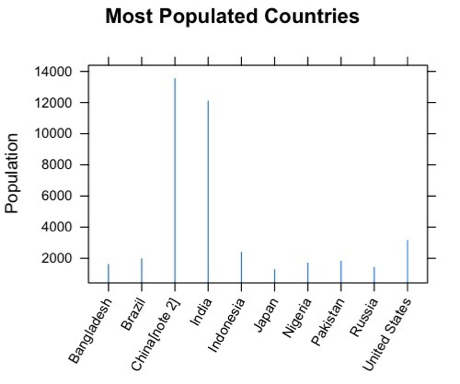
\includegraphics{../IMG/world.png}
\end{center}
\end{frame}

% Finding documentation

\begin{frame}[fragile]
\frametitle{Reading External Files}
Here is a summary of tools to read in various external files, other statistical package formats, and relational databases:
\newline
\footnotesize

\begin{tabular}{| l | l |}
  \hline         
  \textbf{Package/Function} & \textbf{Description} \\ \hline
  readxl & Reads Excel Worksheets and Workbooks \\ \hline
  gdata  & Reads Excel Worksheets and Workbooks    \\ \hline
  XLConnect & Reads Excel Worksheets and Workbooks \\ \hline
   RODBC & Reads Excel Worksheets and Workbooks  \\ \hline
  reader & Read flat/tabular text files from disk \\ \hline
  read.table & Read tabular data from disk \\ \hline
  read.csv & Read tabular data from disk  \\ \hline
  fread & Read large data files from disk  \\ \hline
  haven & Import SAS, STATA, and SPSS files \\ \hline
  foreign & Import SAS, STATA, SPSS, Systat, and Weka files \\ \hline
  RMySQL & Connect to MySQL Databases \\ \hline
  ROracle & Connect to Oracle Databases \\ \hline
  RPostgres & Connect to Postgres Databases \\ \hline
  \hline  
\end{tabular}

\end{frame}

%
\subsection{Reading SAS Files}

\begin{frame}[fragile]
\frametitle{Reading External Files}
Here is an example of reading a SAS dataset. Note that this is a proprietary binary format used
by SAS although the format can be decoded using functions found in the haven addon package. 
\newline
\tiny
\begin{verbatim}
# SAS datsets can be found at http://www.stats.ox.ac.uk/pub/datasets/csb/
# For a list of cool places to find interesting data look at 
# https://catalog.data.gov/dataset?groups=education2168#topic=education_navigation
# http://www.census.gov/programs-surveys/acs/news/data-releases.html
# https://github.com/caesar0301/awesome-public-datasets

library(haven)

sasdataset <- "http://www.principlesofeconometrics.com/poe4/data/sas/lasvegas.sas7bdat"

las_vegas_loans <- read_sas(sasdataset)

head(las_vegas_loans)
  LVR REF INSUR   RATE AMOUNT CREDIT TERM ARM DELINQUENT
1  80   0     1  6.355 1.5760    532   30   1          0
2  89   1     1  6.875 3.1595    703   30   1          0
3  80   1     1  7.080 1.7600    648   30   1          0
4  80   0     0 12.855 1.9680    599   30   1          1
5  70   1     0  5.760 1.8620    626   30   1          0
6  80   0     1  5.555 2.0800    742   30   1          0

\end{verbatim}
\end{frame}
%

\subsection{Reading Excel Files}
\begin{frame}[fragile]
\frametitle{Reading Excel Files}
It is possible to read an Excel spreadsheet although the best thing to do is to first save the spreadsheet into a .csv file and then import it into R using \textbf{read.table()} function.
However, you can read the spreadsheet directly from a file using the add on \textbf{RODBC} package.
\footnotesize
\begin{verbatim}
library(RODBC)

channel <- odbcConnectExcel("examp.xls")

## list the spreadsheets
sqlTables(channel)
  TABLE_CAT TABLE_SCHEM TABLE_NAME TABLE_TYPE REMARKS
1 C:\\bdr NA Sheet1$ SYSTEM TABLE NA
2 C:\\bdr NA Sheet2$ SYSTEM TABLE NA
3 C:\\bdr NA Sheet3$ SYSTEM TABLE NA
4 C:\\bdr NA Sheet1$Print_Area TABLE NA

## retrieve the contents of sheet 1, by either of

sh1 <- sqlFetch(channel, "Sheet1")
sh1 <- sqlQuery(channel, "select * from [Sheet1$]")
\end{verbatim}
\end{frame}


\begin{frame}[fragile]
\frametitle{Reading Files from Other Packages}
R can process XML files which is a format that underlies many websites that distribute interesting data. As an example we can use R and XML to ``geocode'' cities. 
\footnotesize
\begin{center}
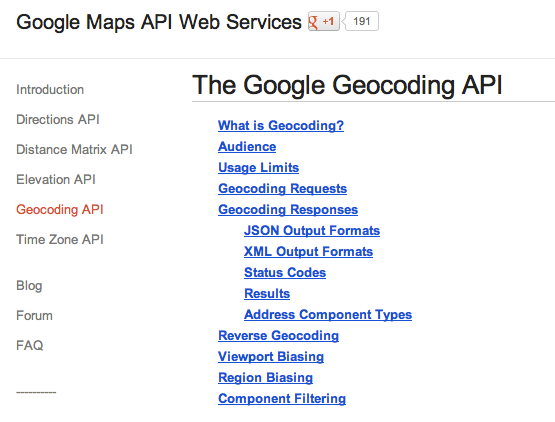
\includegraphics[height=6cm]{../IMG/geocode.png}
\end{center}
\scriptsize
\url{https://developers.google.com/maps/documentation/geocoding/}
\end{frame}

\begin{frame}[fragile]
\frametitle{Reading XML}
\begin{center} 
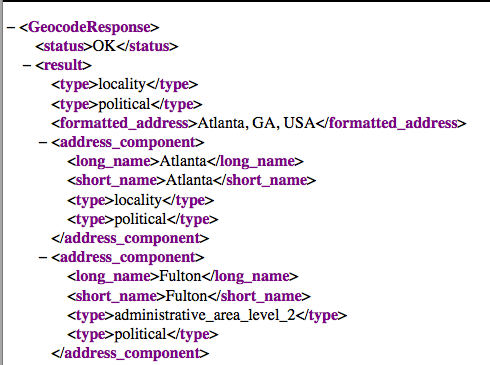
\includegraphics{../IMG/xml.png}
\end{center}
\end{frame}

\begin{frame}[fragile]
\frametitle{Reading XML}
As an example we'll get the latitude and longitude corresponding to the city of Atlanta, Georgia 
\scriptsize
\begin{verbatim}
library(RCurl)
library(XML)

my.url <- "http://maps.googleapis.com/maps/api/geocode/xml?
address <- Atlanta,GA&sensor=false"
txt <- getURL(my.url)
hold <- xmlTreeParse(txt,useInternalNodes=TRUE)

hold
<?xml version="1.0" encoding="UTF-8"?>
<GeocodeResponse>
<status>OK</status>
<result>
<type>locality</type>

place <- getNodeSet(hold,"//GeocodeResponse/result[1]/geometry/location[1]/*")
as.numeric(sapply(place,xmlValue))
[1] 33.74900 -84.38798
\end{verbatim}
\end{frame}



\section{Sinking Your Work}

\begin{frame}[fragile]
\frametitle{Sinking Your Work}
\small
You can capture the output of your work using the \textbf{save()} function. But you can use the \textbf{cat}, \textbf{write} to print out variable values as your code executes. 
\newline
\\
But you can also \textbf{sink} or dump variable values into a file for later inspection. Let's say we have the following code.

\begin{verbatim}
set.seed(123)
x <- rnorm(10)
y <- rnorm(10)

print(x)
cat("y =", y, "\n")

t.test(x,y)
plot(x,y)
\end{verbatim}
The output from this code is on the next slide
\end{frame}


\begin{frame}[fragile]
\frametitle{Sinking Your Work}

\scriptsize
\begin{verbatim}
set.seed(123)
x <- rnorm(10)
y <- rnorm(10)

print(x)
[1] -0.56047565 -0.23017749 1.55870831 0.07050839 0.12928774 1.71506499
[7] 0.46091621 -1.26506123 -0.68685285 ‐0.44566197

cat ("y =", y, "\n")
y = 1.224082 0.3598138 0.4007715 0.1106827 ‐0.5558411 1.786913 0.4978505 
   -1.966617 0.7013559 -04727914

t.test(x,y)
     Welch Two Sample t-?‐test
data: x and y
t = -0.3006, df = 17.872, p-value = 0.7672
alternative hypothesis: true difference in means is not equal to 0
95 percent confidence interval:
-1.0710488 0.8030562
sample estimates:
mean of x mean of y
0.07462564 0.20862196
\end{verbatim}

\end{frame}


\begin{frame}[fragile]
\frametitle{Sinking Your Work}
If desired we could redirect all the output from the print, cat, t.test to a file.
When we run the following we don't see any output. To see the output we have to look at the file \texttt{my.results.txt}

\footnotesize
\begin{verbatim}
sink("my.results.txt") # All output will now go to "my.results.txt"

set.seed(123)
x <- rnorm(10)
y <- rnorm(10)

print(x)

cat ("y =", y, "\n")

t.test(x,y)

plot(x,y)

sink()     # This will deactivate the redirection
\end{verbatim}

\end{frame}

\begin{frame}[fragile]
\frametitle{Sinking Your Work}
Check out the file my.results.txt Note that any graphics files created by the plot command will go into a file called Rplots.pdf
\footnotesize
\begin{verbatim}
$ more my.results.txt
[1] -0.56047565 -0.23017749 1.55870831 0.07050839 0.12928774 1.71506499
[7] 0.46091621 -1.26506123 -0.68685285 -0.44566197
y = 1.224082 0.3598138 0.4007715 0.1106827 -0.5558411 1.786913 0.4978505
-1.966617 0.7013559 -0.4727914

Welch Two Sample t-test

data: x and y
t = -0.3006, df = 17.872, p-value = 0.7672
alternative hypothesis: true difference in means is not equal to 0
95 percent confidence interval:
  -1.0710488 0.8030562
sample estimates:
  mean of x mean of y
0.07462564 0.20862196
\end{verbatim}
\end{frame}


\begin{frame}[fragile]
\frametitle{Sinking Your Work}
If you want more control of the format of the plot output then you can use one of the functions desgined to create plots in a known format (PNG, JPEG, PDF).
\footnotesize
\begin{verbatim}
set.seed(123)
x <- rnorm(10)
y <- rnorm(10)

print(x)
cat ("y =", y, "\n")

t.test(x,y)

pdf("myplots.pdf") # Redirects plots to myplots.pdf

plot(x,y)

dev.off() # Turns off plot redirection
\end{verbatim}
\end{frame}


%%% End of document
\end{document}
